\documentclass[10pt]{amsart}
\usepackage{amsmath,amsthm,amssymb,amsfonts,enumerate,mymath,mathtools,tikz}
\usetikzlibrary{shapes}

\openup 5pt
\author{Blake Farman\\University of South Carolina}
\title{Math 702:\\Homework 03}
\date{February 13, 2013}
\pdfpagewidth 8.5in
\pdfpageheight 11in
\usepackage[margin=1in]{geometry}

\begin{document}
\maketitle

\providecommand{\p}{\mathfrak{p}}
\providecommand{\m}{\mathfrak{m}}

\newtheorem{thm}{}
\newtheorem{lem}{Lemma}

\newcommand{\End}[2]{\operatorname{End}_{#1}\left(#2\right)}
\newcommand{\Hom}[2]{\operatorname{Hom}_{#1}\left(#2\right)}

\begin{thm}
  Determine the splitting field and its degree (over $\Q$) for the following polynomials.
  \begin{enumerate}[(a)]
  \item
    $f(x) = x^4 - 2$
  \item
    $f(x) = x^4 + 2$
  \item
    $f(x) = x^4 + x^2 + 1$
  \item
    $f(x) = x^6 - 4$
  \end{enumerate}
  
  \begin{proof}
    \begin{enumerate}[(a)]
    \item
      The roots for $f$ are $\sqrt[4]{2},\, i\sqrt[4]{2},\, -\sqrt[4]{2},\, \text{and}\ -i\sqrt[4]{2}$ and so $f$ is irreducible over $\Q[x]$.
      Hence the splitting field is $\Q(\sqrt[4]{2}, i\sqrt[4]{2}, -\sqrt[4]{2}, -i\sqrt[4]{2}) = \Q(i,\sqrt[4]{2})$.
      Since $\Q(\sqrt[4]{2})$ is a real field of degree 4, $\Q(i,\sqrt[4]{2}) = \Q(\sqrt[4]{2})(i)$ is a degree 8 extension of $\Q$.
    \item
      Let $\zeta = e^{2\pi i/8}$.
      The roots for $f$ are $\zeta\sqrt[4]{2},\, \zeta^3\sqrt[4]{2},\, \zeta^5\sqrt[4]{2},\, \text{and}\ \zeta^7\sqrt[4]{2}$.
      Hence the splitting field is $K = \Q(\zeta\sqrt[4]{2}, \zeta^3\sqrt[4]{2}, \zeta^5\sqrt[4]{2},\zeta^7\sqrt[4]{2}) \subseteq \Q(i,\sqrt[4]{2})$, which follows from $$\zeta = \frac{\sqrt{2}}{2}(1 + i) = \frac{(\sqrt[4]{2})^2}{2}(1 + i).$$
      To see the reverse containment, first observe that $\sqrt{2} = (\zeta\sqrt[4]{2})(\zeta^7\sqrt[4]{2}) \in K$ and $i = (\zeta\sqrt[4]{2})^2/\sqrt{2} \in K$.
      Hence $\zeta = \sqrt{2}/2(1 + i) \in K$ implies $\sqrt[4]{2} = \zeta\sqrt[4]{2}/\zeta \in K$, completing the reverse containment.
      Therefore $K = \Q(i, \sqrt[4]{2})$.
    \item
      Let $\rho = e^{2\pi i/3} = (-1 + i\sqrt{3})/2$, then observe that $\rho^2 = \overline{\rho} = (-1 - i\sqrt{3})/2$ and $\overline{\rho}^2 = \rho$.
      Factor $f(x) = (x^2 - x + 1)(x^2 + x + 1)$.
      Then $$\rho^2 + \rho + 1 = \overline{\rho} + \rho + 1 = 2\real{\rho} + 1 = -1 + 1 = 0$$ and $$\overline{\rho}^2 + \overline{\rho} + 1 = \rho + \overline{\rho} + 1 = 0$$
      show that $-\rho, -\overline{\rho}, \rho, \overline{\rho}$ are the roots of $x^2 - x + 1$ and $x^2 + x + 1$, respectively.
      Therefore $K = \Q(i\sqrt{3})$ is the splitting field for $f$ and has degree 2 over $\Q$.
    \item
      Factor $x^6 - 4 = {\left(x^{3} - 2\right)} {\left(x^{3} + 2\right)}$.
      Let $\zeta = e^{2\pi i/6} = (1 + i\sqrt{3})/2$ and $\rho = e^{2\pi i/3} = (-1 + i\sqrt{3})/2 = \zeta^2$.
      Then the roots are $\sqrt[3]{2},\, \rho\sqrt[3]{2},\, \overline{\rho}\sqrt[3]{2},\, \zeta\sqrt[3]{2},\, \zeta^3\sqrt[3]{2},\, \text{and}\ \zeta^5\sqrt[3]{2}$.
      The splitting field is 
      $$K = \Q(\sqrt[3]{2}, \rho\sqrt[3]{2}, \overline{\rho}\sqrt[3]{2}, \zeta\sqrt[3]{2}, \zeta^3\sqrt[3]{2}, \zeta^5\sqrt[3]{2}) \subseteq \Q(\sqrt[3]{2}, i\sqrt{3}).$$
      To see the reverse inclusion, observe that $\zeta = \zeta\sqrt[3]{2}/\sqrt[3]{2},\, \rho = \rho\sqrt[3]{2}/\sqrt[3]{2}\in K$ and so $i\sqrt{3} = \zeta + \rho \in K$.
      Then since $F = \Q(\sqrt[3]{2})$ is a real field of degree 3, $K = F(i\sqrt{3})$ is a degree 2 extension of $F$.
      Therefore $K$ is a degree 6 extension of $\Q$.
    \end{enumerate}
  \end{proof}
\end{thm}

\begin{thm}
  Let $p$ be prime, and let $a \neq 0$ in $\F_p$.
  Prove that $x^p - x + a$ is irreducible in $\F_p[x]$ and separable over $\F_p$.
  \begin{proof}
    Let $\alpha$ be a root of $f$.
    Observe that for each $\beta \in \F_p$, $f(\beta) = \beta^p - \beta + a = \beta - \beta + a = a$ and hence $\alpha \not \in \F_p$.
    Moreover,
    $$f(\alpha + \beta) = (\alpha + \beta)^p - (\alpha + \beta) + a = (\alpha^p - \alpha + a) + (\beta - \beta) = 0$$
    implies that $R = \left\{\alpha, \alpha + 1, \ldots, \alpha + (p-1)\right\}$ are all the roots of $f$.
    
    Suppose to the contrary that $f = f_1f_2$ for some $f_1, f_2 \in \F_p[x]$, each of degree at least 1.
    Since $\F_p$ is a field, for each $r \in R$, either $f_1(r) = 0$ or $f_2(r) = 0$.
    Let $S \subseteq R$ be such that $f_1(s) = 0$ for each $s \in S$ and let $n = \abs{S}$.
    Note that $n < p$ since $f_1f_2$ was supposed to be a non-trivial factorization of $f$.
    Write $s_k = \alpha + \beta_k$ for some $\beta_k \in \F_p$, $1 \leq k \leq n$, and $\beta_k = \beta_\ell$ if and only if $k = \ell$.
    Then $f_1(x) = \prod_{k=1}^n (x - (\alpha + \beta_k)) \in \F_p[x]$.
    Consider the coefficient of $x^{n-1}$, 
    $$a_{n-1} = - \sum_{k=1}^n (\alpha + \beta_k) = - n\alpha - \sum_{k=1}^n \beta_k \in \F_p.$$
    Then, since $n < p$, it follows that $\alpha = -(a_{n-1} + \sum_{k=1}^n \beta_k)/n \in \F_p$, a contradiction.
    Therefore $f$ is irreducible.
    
  \end{proof}
\end{thm}

\begin{thm}
  Let $p$ be prime, and let $n \geq 1$.
  Prove that 
  $$x^{p^n - 1} - 1 = \prod_{\alpha \in \F_{p^n}^\times}(x - \alpha).$$
  Conclude that 
  $$\prod_{\alpha \in \F_{p^n}^\times} \alpha = (-1)^{p^n} = \left\{\begin{array}{lr}
  1 & \text{if}\ p = 2,\\
  -1 & \text{if}\ p > 2.
  \end{array}
  \right.$$
  For $p > 2$ and $n = 1$, derive {\bf Wilson's Theorem}: $(p - 1)! \equiv -1 \pmod{p}$.
  \begin{proof}
    Let $f(x) = x^{p^n - 1} - 1 \in \F_{p^n}[x]$.
    For each $\alpha \in \F_{p^n}^\times$, it follows from Lagrange's Theorem that $\alpha^{p^n - 1} = 1$ and so $f(\alpha) = 0$.
    Hence 
    $$f(x) = \prod_{\alpha \in \F_{p^n}^\times}(x - \alpha).$$
    Moreover, comparing constant coefficients for the left- and right-hand sides we have
    $$-1 = \prod_{\alpha \in \F_{p^n}^\times} -\alpha = (-1)^{p^n - 1} \prod_{\alpha \in \F_{p^n}^\times} \alpha.$$
    Hence $$\prod_{\alpha \in \F_{p^n}^\times} \alpha = (-1)^{p^n} = \left\{\begin{array}{lr}
  1 & \text{if}\ p = 2,\\
  -1 & \text{if}\ p > 2.
  \end{array}
  \right.$$
  When $p > 2$ and $n = 1$, we have
  $$-1 = \prod_{\alpha \in \F_{p}^\times} -\alpha = \prod_{\alpha \in \F_{p}^\times} (p - \alpha) = (p - 1)(p - 2)\ldots 1 = (p-1)!.$$
  Therefore $(p-1)! \equiv -1 \pmod{p}$, as desired.
  \end{proof}
\end{thm}

\begin{thm}
  Determine all fields $F$ with $\Q \subseteq F \subseteq \Q(i,\sqrt[4]{3})$.
  Draw a diagram to indicate all containments and degrees of extensions.
  \begin{proof}
    The subfields of $K = \Q(i, \sqrt[4]{3})$ are indicated in the diagram below.
    \begin{center}
      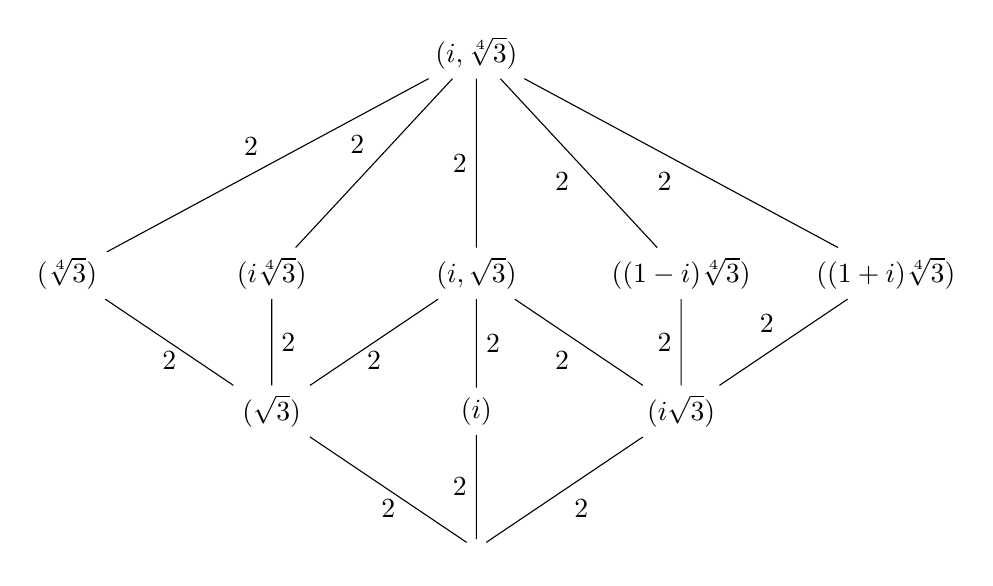
\begin{tikzpicture}[auto, xscale=.65, yscale=.35]
        \node(octic) at (8,23){$\Q(i, \sqrt[4]{3})$};
        \node(quart1) at (0,15){$\Q(\sqrt[4]{3})$};
        \node(quart2) at (4,15){$\Q(i\sqrt[4]{3})$};
        \node(quart3) at (8,15){$\Q(i, \sqrt{3})$};
        \node(quart4) at (12,15){$\Q((1 - i)\sqrt[4]{3})$};
        \node(quart5) at (16,15){$\Q((1 + i)\sqrt[4]{3})$};
        \node(quad1) at (4,10){$\Q(\sqrt{3})$};
        \node(quad2) at (8,10){$\Q(i)$};
        \node(quad3) at (12,10){$\Q(i\sqrt{3})$};
        \node(q) at (8,5){$\Q$};
        \draw (quad1) to node [below] {2} (q);
        \draw (quad2) to node [swap] {2} (q);
        \draw (quad3) to node {2} (q);
        \draw (quad1) to node [below] {2} (quart1);
        \draw (quad1) to node [swap] {2} (quart2);
        \draw (quad1) to node [below] {2} (quart3);
        \draw (quad2) to node [swap] {2} (quart3);
        \draw (quad3) to node {2} (quart3);
        \draw (quad3) to node {2} (quart4);
        \draw (quad3) to node {2} (quart5);
        \draw (quart1) to node {2} (octic);
        \draw (quart2) to node {2} (octic);
        \draw (quart3) to node {2} (octic);
        \draw (quart4) to node {2} (octic);
        \draw (quart5) to node {2} (octic);
      \end{tikzpicture}
    \end{center}
    The containments for the quadratic extensions follow from the fact that $i, \sqrt{3} = (\sqrt[4]{3})^2, i\sqrt[4]{3} \in K$.
    The containments of the other quartic extensions $\Q(i,\sqrt{3})/\Q$, $\Q(\sqrt[4]{3})/\Q$, $\Q(i\sqrt[4]{3})/\Q$, and $\Q((1 \pm i)\sqrt[4]{3})/\Q$ follow similarly.
    That $\Q((1 \pm i)\sqrt[4]{3})/\Q$ are quartic extensions follows from the fact that 
    $$x^4 + 12 = {\left(x - \left(i - 1\right) \, \sqrt[4]{3}\right)}
    {\left(x + \left(i - 1\right) \, \sqrt[4]{3}\right)}
    {\left(x + \left(i + 1\right) \, \sqrt[4]{3}\right)}
    {\left(x - \left(i + 1\right) \, \sqrt[4]{3}\right)},$$
    which is Eisenstein in 3.
    Their containment of $\Q(i\sqrt[4]{3})$ follows from 
    $$i\sqrt{3} = -((1-i)\sqrt[4]{3})^2/2 = ((1+i)\sqrt[4]{3})^2/2.$$
    That $\Q(\sqrt[4]{3})/\Q$ and $\Q(i\sqrt[4]{3})/\Q$ are quartic extensions follows from the fact that they are roots of the irreducible polynomial $x^4 - 3$.
    Both clearly contain $\sqrt{3} = (\sqrt[4]{3})^2 = -(i\sqrt[4]{3})^2$.
    That $\Q(i, \sqrt{3})/\Q$ is a quartic extension follows from the fact that $\pm i$ is not contained in the real field $\Q(\sqrt{3})$ and so $\Q(\sqrt{3})(i) = \Q(i,\sqrt{3})$ has degree four over $\Q$.
  \end{proof}
\end{thm}

\begin{thm}
  Let $F$ be a field, and for all $j \geq 1$, let $\mu_j$ denote the $j^\text{th}$ roots of unity.
  \begin{enumerate}[(a)]
    \item
      Let $n \geq 1$ be odd, and suppose that $\mu_n \subseteq F$.
      Prove that $\mu_{2n} \subseteq F$.
    \item
      Let $k, m, p \geq 1$ with $p$ prime and $p \nmid m$.
      Suppose that $n = p^km$ and that $\operatorname{char} F = p$.
      Prove that $x^n - 1 \in F[x]$ has $m$ distinct roots in a splitting field.
      In other words, the number of $n^\text{th}$ roots of unity over a field of characteristic $p$ is $n/p^{v_p(n)}$.
    \item
      Let $n > 1$ be odd.
      Prove that $\Phi_{2n}(x) = \Phi_n(-x)$.
  \end{enumerate}

  \begin{proof}
    \begin{enumerate}[(a)]
    \item\label{5.a}
      First note that since $\mu_n \subseteq F$, $x^{n} - 1$ is separable and so it follows that $x^n + 1$ is also separable.
      Observe that $f(x) = x^{2n} - 1 = (x^n + 1)(x^n - 1)$.
      %Since $D_x  (x^{2n} - 1) = 2nx^{2n - 1}$ and 0 is not a root of $x^{2n} - 1$, it follows that $\gcd(x^{2n} - 1, D_x (x^{2n} - 1))= 1$.
      %Hence $x^{2n} - 1$ is separable.
      If $\zeta \in \mu_n$, then $\zeta^n - 1 = 0$ implies that $f(\zeta) = 0$ and thus $\zeta \in \mu_{2n}$.
      Moreover, $0 = -\zeta^n + 1 = (-\zeta)^n + 1$ shows that $-\zeta \in \mu_{2n}$.
      Note that $-\zeta \not \in \mu_n$, for otherwise $(-\zeta)(\zeta^{n-1}) = -1 \not \in \mu_n$.
      Hence, by uniqueness of inverses, these are the $2n$ roots of $x^{2n} - 1$, each in $F$.
      Therefore $\mu_{2n} \subseteq F$, as desired.
    \item\label{5.b}
      Since $\operatorname{char} F = p$, we may rewrite $x^n - 1 = (x^m)^{p^k} + (-1)^{p^k} = (x^m - 1)^{p^k}$.
      Then the $n^{th}$ roots of unity in $F$ are precisely the $m^{\text{th}}$ roots of unity.
      To see that there are $m$ roots of $x^m - 1$, consider $D_x(x^m - 1) = mx^{m-1}$.
      Since $p \nmid m$, zero is the only root, with multiplicity $m - 1$, and so $\gcd(mx^{m-1}, x^m - 1) = 1$.
      Therefore $x^m - 1$ is separable, as desired.
    \item\label{5.c}
      Let $\zeta$ be a primitive $n^{th}$ root of unity.
      Observe that, by part~\eqref{5.a}, $-\zeta$ is a $2n^\text{th}$ root of unity and its order must necessarily be $2n$, since in $\mu_{2n}$, $\operatorname{o}(-1) = 2$, $\operatorname{o}(\zeta) = n$ and $\gcd(2,n) = 1$.
      Hence $-\zeta$ is a primitive $2n^\text{th}$ root of unity.
      Then write 
      $$\Phi_n(x) = \prod_{\substack{1 \leq a \leq {n-1}\\a \nmid n}}(x - \zeta^a)$$
      so that
      $$\Phi_n(-x) = \prod_{\substack{1 \leq a \leq {n-1}\\a \nmid n}}(-x - \zeta^a) = (-1)^{\phi(n)} \prod_{\substack{1 \leq a \leq {n-1}\\a \nmid n}}(x - (-\zeta^a)) = \prod_{\substack{1 \leq a \leq {n-1}\\a \nmid n}}(x - (-\zeta^a)),$$
      where the last equality follows from the fact that $\phi(n)$ is even for all $n \geq 3$.
      Since $\gcd(2,n) = 1$ and $\phi$ is multiplicative, we have that $$\deg{\Phi_{2n}(x)} = \phi(2n) = \phi(2)\phi(n) = \phi(n) = \deg{\Phi_n(x)}.$$
      Since $-\zeta$ is a root of $\Phi_n(-x)$, we have that $\Phi_{2n}(x)$, the minimal polynomial for $-\zeta$, divides $\Phi_n(-x)$.
      However $\Phi_n(-x)$ and $\Phi_{2n}(x)$ are both monic, of the same degree.
      Therefore $\Phi_n(-x) = \Phi_{2n}(x)$.
    \end{enumerate}
  \end{proof}
\end{thm}

\begin{thm}
  Let $p \neq \ell$ be primes, and let $f$ be the order of $p$ in $(\Z/\ell\Z)^\times$ (i.e. $f$ is the least positive integer with $p^f \equiv 1 \pmod{\ell}$).
  Let $\zeta$ be a root of $\Phi_\ell(x) \in \F_p[x]$.
  \begin{enumerate}[(a)]
   \item\label{6.a}
     Use that $\F_{p^n}^\times$ is cyclic to prove that the least positive integer $n$ with $\zeta \in \F_{p^n}$ is $n = f$.
     Conclude that the minimal polynomial of $\zeta$ over $\F_p$ has degree $f$.
   \item
     Let $a \in \Z$ with $\ell \nmid a$.
     Prove that $\F_p(\zeta) = F_p(\zeta^a)$ [One inclusion is obvious.
       For the other, note that $\zeta = (\zeta^a)^b$ where $ab \equiv 1 \pmod{\ell}$].
     Use \eqref{6.a} to show that $\Phi_\ell(x)$ factors into a product of $\frac{\ell - 1}{f}$ disctinct irreducible polynomials, each of degree $f$.
  \end{enumerate}
  
  \begin{proof}
    \begin{enumerate}[(a)]
        \item
          By assumption, $\zeta$ is a primitive $\ell^\text{th}$ root of unity, and so if $\zeta \in \F_{p^n}$, then its order must be $\ell$.
          By virtue of $\F_{p^n}^\times$ being cyclic of order $p^n - 1$, $\ell$ divides $p^n - 1$.
          Hence if $\zeta \in \F_{p^n}^\times$, then $n \geq f$.
          
          Now consider $\F_{p^f}^\times$.
          Let $g$ generate $\F_{p^f}^\times$.
          Since $\ell$ divides $p^f - 1$, we have that $g^{(p^f - 1)/\ell}$ is an element of order 
          $$\frac{p^f - 1}{\gcd(p^f - 1, \frac{p^f - 1}{\ell})} = \ell.$$
          Hence $\zeta \in \F_{p^f}$.
          Therefore by minimality of $\F_p(\zeta)$ and uniqueness of finite fields, $\F_{p^f} \cong \F_p(\zeta) \cong F_{p}[x]/(m_{\zeta,\F_p})$ and $\deg{m_{\zeta,\F_p}} = f$, as desired.
        \item
          Since $a$ does not divide $\ell$, $a$ is invertible modulo $\ell$.
          Let $b$ be an integer such that $ab \equiv 1 \pmod{\ell}$.
          Then $\zeta = (\zeta^a)^{b} \in F(\zeta^a)$ yields the inclusion $F(\zeta) \subseteq F(\zeta^a)$.
          The reverse inclusion follows from $\zeta^a = (\zeta)^a \in F(\zeta)$.
          Hence for each such $a$, $\zeta^a$ is a primitive $\ell^\text{th}$ root of unity and $\zeta^a$ is the root of $\Phi_\ell(x)$.
          It then follows that the minimal polynomial of $\zeta^a$ divides $\Phi_\ell(x)$.
          Therefore by part~\eqref{6.a}, $\Phi_\ell(x)$ factors into the product of $\frac{\ell - 1}{f}$ distinct irreducibles, each of degree $f$.
    \end{enumerate}    
  \end{proof}
\end{thm}

\end{document}
